\documentclass[14pt, fleqn, xcolor={dvipsnames, table}]{beamer}
\usepackage[T2A]{fontenc}
\usepackage[utf8]{inputenc}
\usepackage[english,russian]{babel}
\usepackage{amssymb,amsfonts,amsmath,mathtext}
\usepackage{cite,enumerate,float,indentfirst}
\usepackage{cancel}
\usepackage{graphicx}
\usepackage{animate}

\usepackage{tikz}
% \usepackage{enumitem}
\usetikzlibrary{shadows}

% \usepackage{enumitem}
% \setitemize{label=\usebeamerfont*{itemize item}%
%   \usebeamercolor[fg]{itemize item}
%   \usebeamertemplate{itemize item}}

\graphicspath{{images/}}

\usetheme{Madrid}
\usecolortheme{seahorse}
\renewcommand{\CancelColor}{\color{red}}

\setbeamercolor{footline}{fg=Blue!50}
\setbeamertemplate{footline}{
  \leavevmode%
  \hbox{%
  \begin{beamercolorbox}[wd=.333333\paperwidth,ht=2.25ex,dp=1ex,center]{}%
    И. Кураленок, Н. Поваров, Яндекс
  \end{beamercolorbox}%
  \begin{beamercolorbox}[wd=.333333\paperwidth,ht=2.25ex,dp=1ex,center]{}%
    Санкт-Петербург, 2014
  \end{beamercolorbox}%
  \begin{beamercolorbox}[wd=.333333\paperwidth,ht=2.25ex,dp=1ex,right]{}%
  Стр. \insertframenumber{} из \inserttotalframenumber \hspace*{2ex}
  \end{beamercolorbox}}%
  \vskip0pt%
}
\newcommand\indentdisplays[1]{%
     \everydisplay{\addtolength\displayindent{#1}%
     \addtolength\displaywidth{-#1}}}
\newcommand{\itemi}{\item[\checkmark]}

\newenvironment{mydescription}[1]
  {\begin{list}{}%  
   {\renewcommand\makelabel[1]{\color{blue}##1:\hfill}%
   \settowidth\labelwidth{\makelabel{#1}}%
   \setlength\leftmargin{\labelwidth}
   \addtolength\leftmargin{\labelsep}}}
  {\end{list}}

\title{Глубокое обучение\\\small{по Deep Learning Tutorial by Yann LeCun and Marc'Aurelio Ranzato, ICML 2013}}
\author[]{\small{%
И.~Куралёнок,
Н.~Поваров}}
\date{}
\begin{document}

\begin{frame}
\maketitle
\small
\begin{center}
\vspace{-60pt}
\normalsize {\color{red}Я}ндекс \\
\vspace{80pt}
\footnotesize СПб, 2014
\end{center}
\end{frame}
\section{Понятие глубокого обучения} % про сведение решающей функции к комбинации зависимых переменных инженерным способом

\begin{frame}{Глубокое обучение}{Определение по Simona Ullo}
\small
''A \textbf{relatively recently developed}$^1$ set of generative machine learning techniques that \textbf{autonomously}$^2$ generate \textbf{high-level representation}$^3$ from raw data sources, and using these representations can perform typical machine learning tasks such as classification, regression and clustering''\\ 
\begin{enumerate}
\uncover<2->{\item back to 80s: learning neural networks --- multiple layers with non-linear transformations(backpropagation)}
\uncover<3->{\item from hand-crafted features to feature learning}
\uncover<4->{\item hierarchical representation increasing level of abstraction}
\end{enumerate}
\uncover<5->{2 + 3 = automated discovery of abstraction}
\end{frame}
 
\begin{frame}{Что считать достаточно глубоким?}{Известные методы со сложной решающей функцией}
\begin{minipage}{0.45\textwidth}\small
\begin{itemize}
  \item Нейронные сети с 1-м скрытым уровнем
  \item SVM и Kernel методы
  \item Деревья решений
\end{itemize}
\end{minipage}
\hfill
\begin{minipage}{0.45\textwidth}
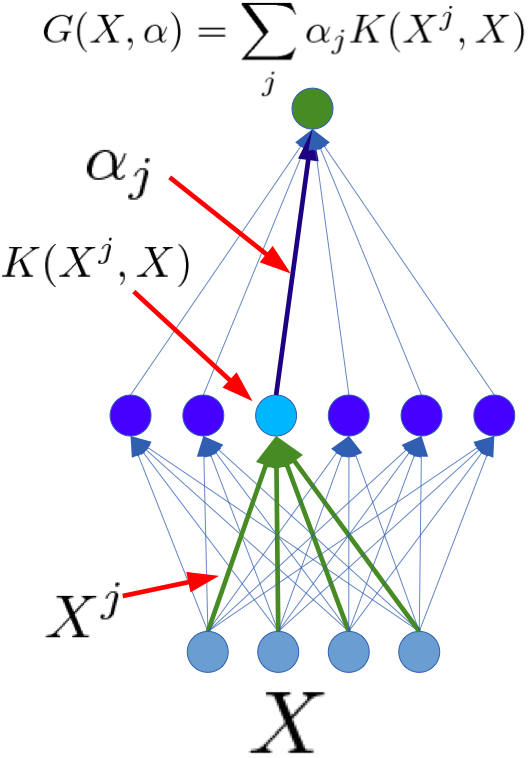
\includegraphics[width=\textwidth]{svmisnotdeep.png}
\end{minipage}
\end{frame}

\begin{frame}{Что считать достаточно глубоким?}{Графические модели}
\small
Графические модели могут быть отнесены к глубокому обучению, однако:
\begin{itemize}
  \item При конструировании графической модели, мы используем топологию, чтобы ``подсказать'' какие факторы можно построить (по сути не сама сеть конструирует факторы, а мы проверяем гипотезу о полезности фактора для данной модели)
  \item GPM можно свести к нейронным сетям аля Больцман (мы уже говорили, что NN --- это язык).
\end{itemize}
\end{frame}

\begin{frame}{Что считать достаточно глубоким?}{Итого}\Large
Будем смотреть только на нейронные сети, так как больше ничего не нашли :)
\end{frame}

\begin{frame}{Какие фичи хорошие?}
\small
\textbf{Пример}\\
Дима и Вячеслав фотографировали друг друга, для размещения в соц сетях. Нафотографировали 1000 фотографий на фоне белой стены. Фотографии $1000\times1000$. Общий объем информации на диске: $1000\cdot1000\times1000\times3 \simeq 3Gb$. А сколько на самом деле там информации?
\uncover<2->{
\begin{itemize}
\item На лице человека $<50$ мышц
\item 3 координаты положения относительно камеры
\item 3 координаты угла поворота
\end{itemize}
$\Rightarrow$ Итого каждая фотография получается из любой другой, зная дополнительные 56 чисел. 
$2 \cdot 1000\times1000\times3 + 998 \cdot 56 \times 4 \simeq 6.2Mb$
}
\end{frame}

\begin{frame}{Какие фичи хорошие?}
\begin{center}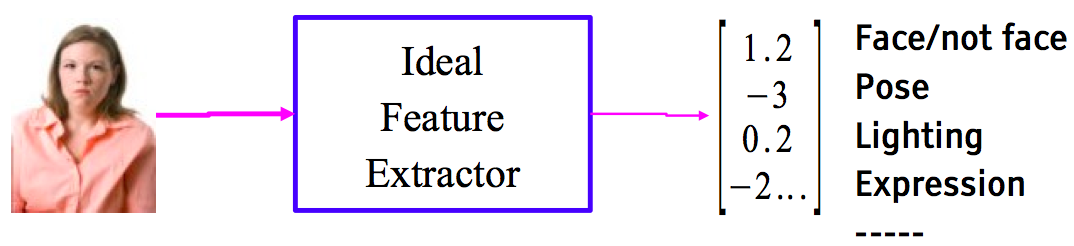
\includegraphics[width=0.8\textwidth]{faces.png}\end{center}
\small
Хотим получить такие фичи. Однако, кажется понятно, что мы вряд ли сможем получить их напрямую из цветов на картинке $\Rightarrow$ нужно уметь вытаскивать ``более высокий уровень абстракции''.\\
На самом деле, мы скорее идем от обратного:
\begin{enumerate}
  \item Хочется, например, узнать закрыты глаза или нет
  \item Линейной комбинацией его предсказать не получается
  \item[$\Rightarrow$] будем надеяться, что получится нелинейно
\end{enumerate}
\end{frame}

\begin{frame}{Идея как сделать инвариантные факторы}
\small
\begin{itemize}
  \item Запихнуть точки в более многомерное пространство так, чтобы была разделимость
  \item Уменьшить размерность так, чтобы разделимость осталась
\end{itemize}
\begin{center}
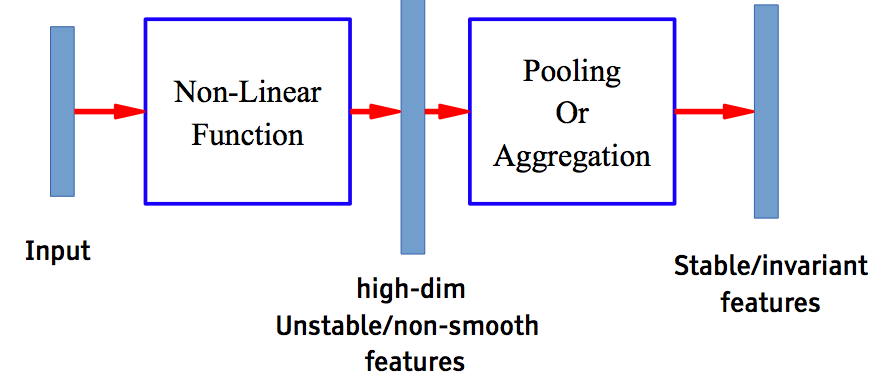
\includegraphics[height=0.4\textheight]{invariantfeaturelearning.png}
\end{center}
\end{frame}

\begin{frame}{Идея как сделать инвариантные факторы}
\begin{center}
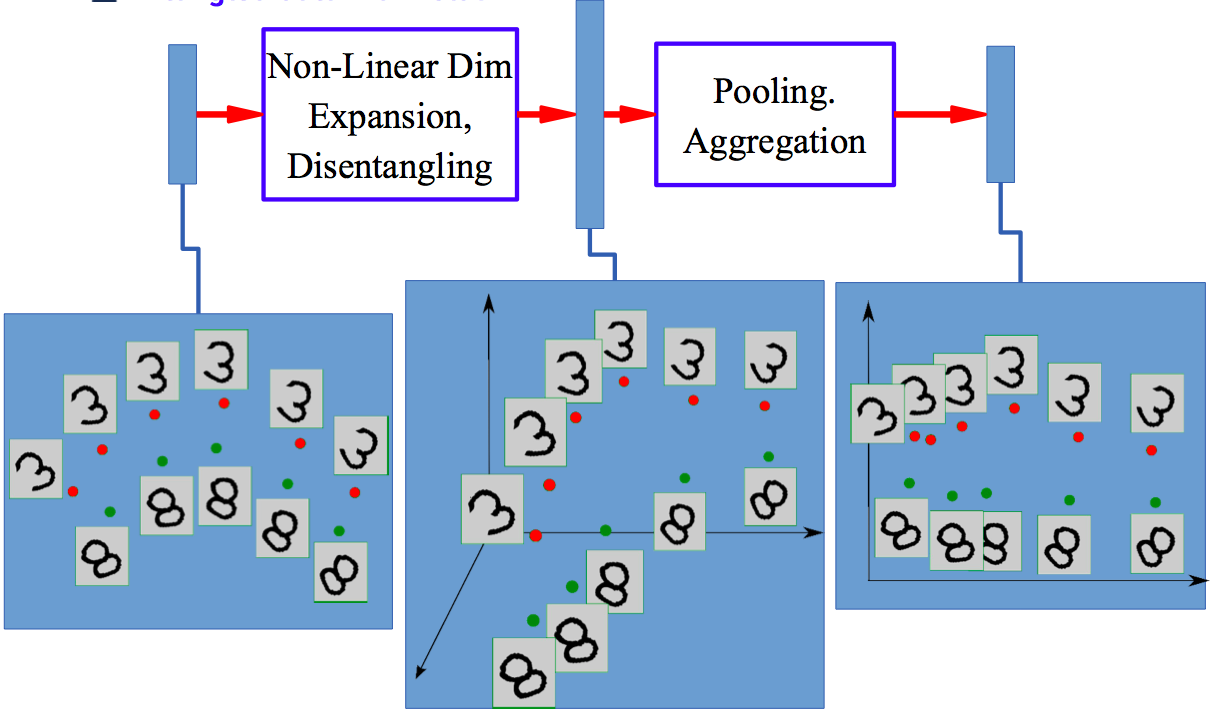
\includegraphics[width=0.9\textwidth]{fullconvcycle.png}
\end{center}
\end{frame}

\begin{frame}{Что такое свертки}{Или как работает Kinect}
\only<1>{
  Есть задачка:
  \begin{center}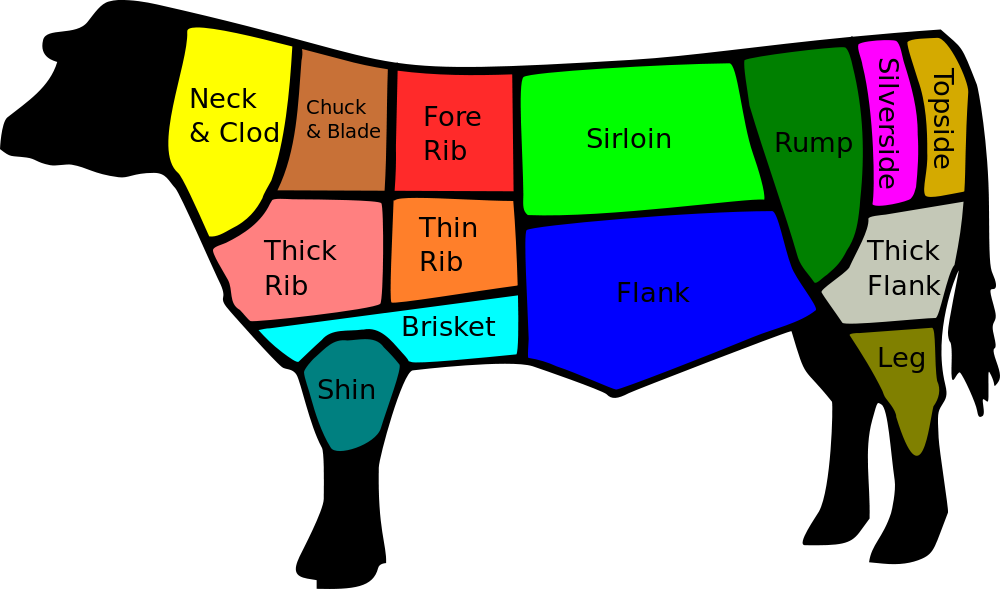
\includegraphics[width=0.9\textwidth]{1000px-British_Beef_Cuts.png}\end{center}
}
\only<2-> {
\textbf{Дано:} Камера, которая умеет мерять глубину, приделанная к телевизору. Много-много (1млн+) размеченных по схеме картинок.\\
\textbf{Найти:} Как расположены по отношении друг к другу topside и neck\\
\textbf{Решение:}\small
\begin{itemize}
\item Возьмем для каждой точки глубину точек вокруг
\item Представим их в качестве вектора
\item По полученному вектору подберем решение (у них деревья, насколько я помню), которое отнесет данную точку к сегменту тела
\item[$\Rightarrow$] Profit!
\end{itemize}
}
\end{frame}

\begin{frame}{Объединим свертки и Deep Learning}
\begin{center}
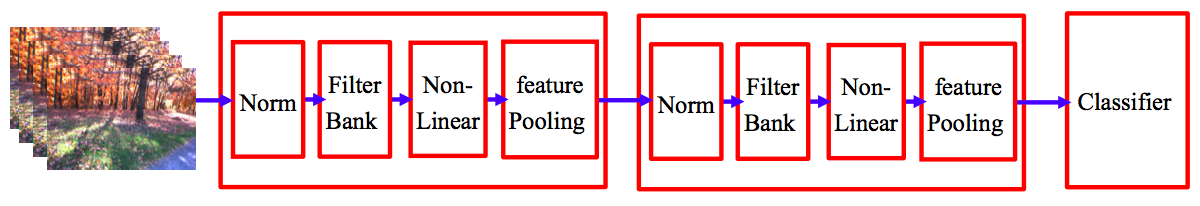
\includegraphics[width=0.9\textwidth]{convolution-scheme.png}
\end{center}
\begin{enumerate}\small
  \item Нормализация (whitening)
  \item Фильтрация (увеличение размерности)
  \item Нелинейное преобразование (tanh, $(1 + e^{-x})^{-1}$, max, ReLU)
  \item Пулинг ($l_q$, $\frac{1}{b}\log\left(\sum_i e^{b x_i}\right)$)
\end{enumerate}
\end{frame}

\begin{frame}{Типы слоев в сверточных сетях}
\begin{center}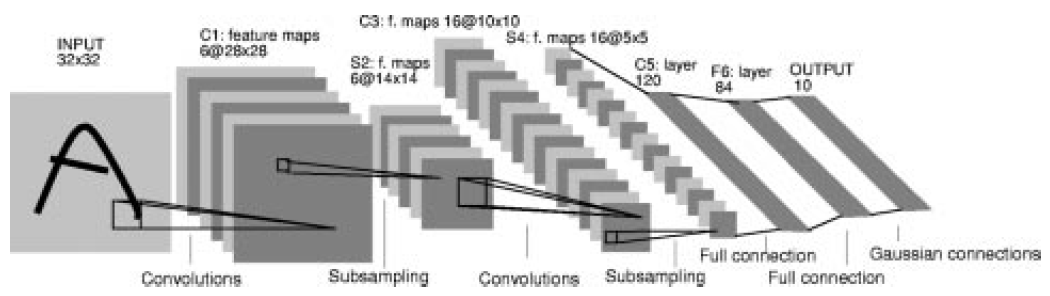
\includegraphics[width=0.9\textwidth]{convnet.png}\end{center}
\begin{itemize}
\item Простая однослойная свертка 
\item Многослойная свертка
\item Pooling/subsampling
\item Сложный персептрон в качестве классификатора
\end{itemize}
% http://citeseerx.ist.psu.edu/viewdoc/download;jsessionid=0D70E2A5D733AADC8DBE9CBCB73FE0AA?doi=10.1.1.138.1115&rep=rep1&type=pdf
\end{frame}

\begin{frame}{Почему все это не переобучается}{адски}
\small
\begin{itemize}
  \item Число связей хоть и велико, но все же не такое большое как в полносвязных слоях
  \item Мы обучаем ``фичи'' почти независимо
  \item Число факторов ``более высокого уровня абстракции'' фиксированно \footnote{грубо говоря у нас жесткое ограничение на число значащих параметров}
  \item Каждая новая фича зависит от большого числа случайных отображений, и мы надеемся на ЗБЧ
\end{itemize}
\end{frame}

\begin{frame}{Dropout}
\small
Если начальные веса рандомны, то при обучении производные будут сильно неравномерны. Это приведет к вырождению связей и небольшому числу эффективных зависимостей $\Rightarrow$ никаких ЗБЧ $\Rightarrow$ Dropout:
\begin{enumerate}
  \item Добавим в вес связи бернуллевскую случайную компоненту
  \item Будем учитывать эту компоненту на этапе обучения (при распространении ошибки) и/или на этапе работы
\end{enumerate}
\end{frame}

\begin{frame}{Известные результаты успешного DL}
\small
\begin{itemize}
  \item Handwriting Recognition and OCR (late 1980s to mid 1990s)\\
\textit{Supervised convolutional nets operating on pixels}
  \item Face \& People Detection (early 1990s to mid 2000s)\\
\textit{Supervised convolutional nets operating on pixels (YLC 1994, 2004, Garcia 2004)}
  \item Low-Res Object Recognition: road signs, house numbers (early 2010's)\\
\textit{Supervised convolutional net operating on pixels}
  \item Speech Recognition II (circa 2011) \\
\textit{Deep neural nets for acoustic modeling}
  \item Object Recognition II, Semantic Labeling (2012, Hinton, YLC,...) \\
\textit{Supervised convolutional nets operating on pixels}
\end{itemize}
\end{frame}

\begin{frame}{Deep learning: что забыли?}
\textbf{\color{blue}Нелинейность:} диалоги о нелинейности до сих пор ведутся, но пока выигрывает ReLU \\
\textbf{\color{blue}Другие виды сетей:} нет им числа: DBN, DBM, любое другое поделие с более 2-х скрытых слоев \\
\textbf{\color{blue}DL как чистый RL:} снимем последний слой сети, и посмотрим как можно использовать получившиеся факторы
\end{frame}

\begin{frame}{Что мы сегодня узнали}
\begin{itemize}
  \item Нейронные сети единственные из известных видов обучения, способные быть ``достаточно глубокими''
  \item В глубоком обучении слои распределяют по ролям
  \item Сверточные сети позволяют использовать связность исходного пространства факторов
  \item Нейронные сети нашли свое применение в картинках и голосе
  \item Есть живые библиотеки, которые можно использовать для DL на дому
\end{itemize}
\end{frame}
\end{document}
